\documentclass{phyasgn}
\phyasgn{
  stuname = 姚昊廷,           % 设置学生姓名
  stunum = 22322091,      % 设置学号
  setasgnnum = 12,           % 设置课程次数
  classname = 电磁学,     % 设置课程名称
}

\usepackage{listings}
\usepackage{tikz}
\usepackage{amssymb}
\usepackage{t-angles}
\usepackage{amssymb}
\usepackage{tikz}
\usepackage{mathrsfs}
%\usepackage{autobreak} 
%\usepackage{fixdif} 
\usetikzlibrary{quotes,angles}
\usetikzlibrary{calc}
\usetikzlibrary{decorations.pathreplacing}
\lstset{numbers=left,basicstyle=\ttfamily,columns=flexible}
\makeatletter
\newcommand{\rmnum}[1]{\romannumeral #1}
\newcommand{\Rmnum}[1]{\expandafter\@slowromancap\romannumeral #1@}
\makeatother


\begin{document}

\begin{sol}[2-43]
$$\frac{1}{2}mv^2=Uq\to v=\sqrt{\frac{2Uq}{m}}$$
$$\begin{aligned}
    qvB&=\frac{mv^2}{r}\\
    qB&=\frac{m\sqrt{\frac{2Uq}{m}}}{\frac{x}{2}}\\
    m&=\frac{qB^2}{8U}x^2
\end{aligned}$$
\end{sol}\par

\begin{sol}[2-45]
    (1)$$\begin{aligned}
        E&=\frac{1}{2}mv^2\\
        v&=\sqrt{\frac{2E}{m}}
    \end{aligned}$$
    $$B=\frac{mv}{qR}=\frac{\sqrt{2mE}}{qR}=0.48\text{T}$$
    (2)$$n=\frac{E}{Uq}=200$$
    $$\begin{aligned}
        F&=ma\\
        \frac{U}{d}q&=ma\\
        a&=\frac{Uq}{md}
    \end{aligned}$$
又因为圆周运动满足$R=\frac{mv}{Bq}$,故运动周期为$$T=\frac{2\pi R}{v}=\frac{2\pi m}{Bq}$$
故$$t=\frac{v}{a}+n\frac{T}{2}=\frac{\sqrt{\frac{2E}{m}}}{\frac{Uq}{md}}+\frac{200\pi m}{Bq}=1.38\times 10^{-5}\text{s}$$
\end{sol}

\begin{sol}[2-50]
    (1)N型\\
    (2)$$\frac{U}{b}e=Bev\to v=\frac{U}{Bb}$$
    $$\begin{aligned}
        I&=neSv\\
        n&=\frac{I}{nev}=\frac{BI}{eaU}=2.9\times 10^{20}\text{/m}^3
    \end{aligned}$$
\end{sol}\par

\begin{sol}[2-50]
    (1)N型\\
    (2)$$\frac{U}{b}e=Bev\to v=\frac{U}{Bb}$$
    $$\begin{aligned}
        I&=neSv\\
        n&=\frac{I}{nev}=\frac{BI}{eaU}=2.9\times 10^{20}\text{/m}^3
    \end{aligned}$$
\end{sol}\par

\begin{sol}[3-5]
    \begin{figure}[h]
        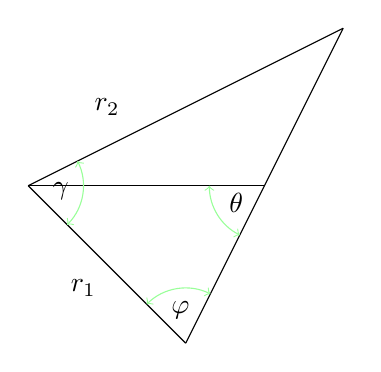
\begin{tikzpicture}
            \coordinate (a) at (3,0);
            \coordinate (b) at (4,2);
            \coordinate (o) at (0,0);
            \coordinate (c) at (2,-2);
            \draw (o) --(a);
            \draw (o) --(b);
            \draw (o) --(c);
            \draw (b) --(c);
            \node at(0.7,-1.3) {$r_1$};
            \node at(1,1) {$r_2$};
            \pic["$\theta$", draw=green!40, <->, angle eccentricity=0.6, angle radius=0.7cm]
        {angle=o--a--c};
        \pic["$\gamma$", draw=green!40, <->, angle eccentricity=0.6, angle radius=0.7cm]
        {angle=c--o--b};
        \pic["$\varphi$", draw=green!40, <->, angle eccentricity=0.6, angle radius=0.7cm]
        {angle=b--c--o};
        \end{tikzpicture}
    \end{figure}
$$\begin{aligned}
    \Phi&=\int \mathbf{B}\cdot \d \mathbf{S}\\
    &=\int_0^{\gamma}2a\frac{r\d \alpha}{\sin\beta}\frac{\mu_0I}{2\pi r}\cos\beta\\
    &=\frac{a\mu_0I}{\pi}\int_0^{\gamma}\frac{\cos\beta\d \alpha}{\sin\beta}
\end{aligned}$$
又因为$\beta=\varphi+\alpha$
故$$\begin{aligned}
    \Phi&=\frac{a\mu_0I}{\pi}\int_\varphi^{\gamma+\varphi}\frac{\cos\beta\d \beta}{\sin\beta}\\
    &=\frac{a\mu_0I}{\pi}\ln\frac{\sin(\varphi+\alpha)}{\sin(\phi)}\\
    &=\frac{a\mu_0I}{2\pi}\ln\frac{r_1}{r_2}\\
    &=\frac{a\mu_0I}{2\pi}\left ( \ln(a^2+b^2-2ab\cos\theta )-\ln (a^2+b^2+2ab\cos \theta ) \right ) 
\end{aligned}$$
故电动势为
$$\begin{aligned}
    \mathscr{E}&=\frac{\d \Phi}{\d t}\\
    &=\frac{\d\Phi}{\d \theta}\frac{\d \theta}{\d t}\\
    &=\frac{-\mu_0Ia^2b\omega\sin(\omega t)}{\pi}\left ( \frac{1}{a^2+b^2+2ab\cos (\omega t)} +\frac{1}{a^2+b^2-2ab\cos (\omega t)} \right ) 
\end{aligned}$$
\end{sol}\par

\begin{sol}[3-8]
    $$\begin{aligned}
        \d Q&=I\d t\\
        \d Q&=\frac{\d \Phi}{R\d t}\d t\\
        \Delta Q&=\frac{\Delta\Phi}{R}\\
        \Delta Q&=\frac{N\pi d^2B}{2R}\\
        B&=\frac{2R\Delta Q}{N\pi d^2}=1.3\times10^{-4}\text{T}
    \end{aligned}$$
\end{sol}\par
\end{document}